\chapter{Test des Algorithmus im Frequenzbereich}\label{appendix:test_algorithmus}

Zum Test der \textit{Output Error}-Methode mit dem \textit{Newton-Raphson}-Algorithmus wurde ein sinusförmiges Signal 
mit einer bestimmten Frequenz in der Höhenruderstuerung sowie ein Sinus-Signal im Anstellwinkel erstellt und der Algorithmus 
verwendet, um die entsprechende Über-tragung zu identifizieren. Mit der 
identifizierten Übertragunsgfunktion wurde dann eine Näherung des 
Zustandsverlaufs berechnet. Wie sich in 
\cref{fig:testdaten1} erkennen lässt, wird die 
ursprüngliche Frequenz gut angenähert. Der Anstellwinkelverlauf wird vom Algorithmus mit einem leichten Phasenversatz noch 
gut getroffen (vgl. \cref{fig:testdaten2}).\par
Die anderen Zustände wurden in diesem Test nicht betrachtet, der Schubdrosselgrad wurde konstant gehalten.

\begin{figure}[!h]
	\centering
	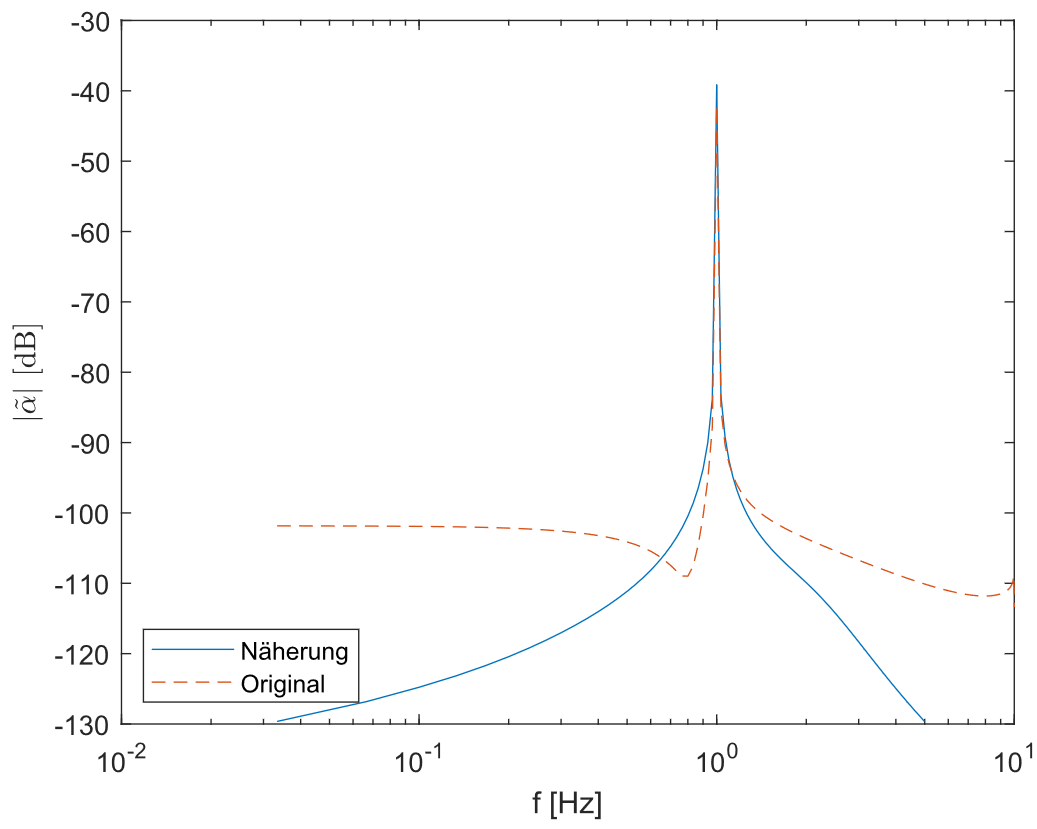
\includegraphics[width=0.6\linewidth]{src/pics/Testdaten1}
	\caption{Betragskennlinie des Originalsignals sowie der Näherung}
	\label{fig:testdaten1}
\end{figure}

\begin{figure}[!h]
	\centering
	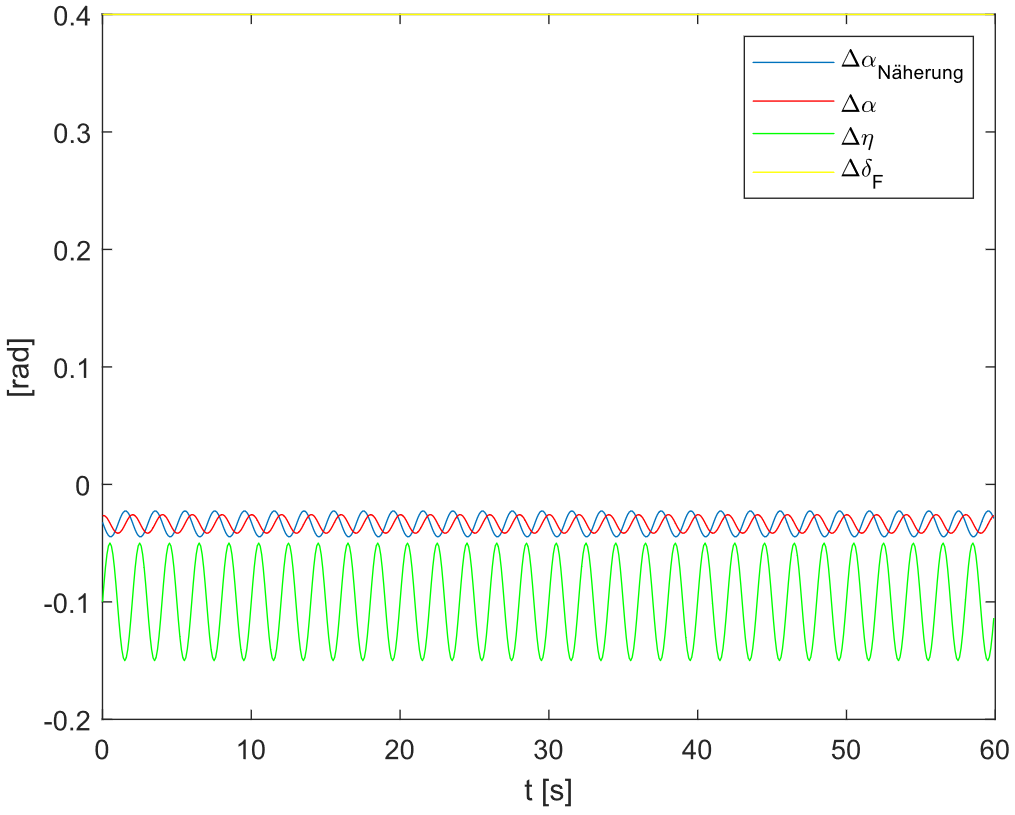
\includegraphics[width=0.6\linewidth]{src/pics/Testdaten2}
	\caption{Zeitverläufe des Originalsignals sowie der Näherung und der 
	Steuerungen}
	\label{fig:testdaten2}
\end{figure}
